% !TEX = root../thesis.tex

\chapter{Experimental Apparatus}
\label{chap:exp}

\section{The Large Hadron Collider} \label{sec:LHC}
% Overview
The Large Hadron Collider (LHC) is a circular collider spanning the border between France and Switzerland, based at the European Organization for Nuclear Research (CERN). The central features of the LHC are the superconducting rings, located about 100 m underground with a circumference of 27 km, designed to collide counter-rotating beams of protons or heavy ions at highly relativistic energies. Along the rings lie four major experiments: ATLAS, CMS, ALICE, and LHCb. Both ALTAS and CMS are general purpose detectors, designed to probe a wide range of physics including the Higgs boson, precision measurements of fundamental constants, and physics beyond the standard model (BSM). The remaining two experiments are more specialized; ALICE measures quark gluon plasma produced in heavy ion collisions and LHCb focuses on $b$-quark physics and CP violation.

% Lumi and CoM energy
Two prominent aspects of the LHC are the high center of mass energy, referred to using the Mandelstam variable $\sqrt{s}$, and high instantaneous luminosity $\lumi$, often referred to as just luminosity. High $\sqrt{s}$ allows for the production of more massive particles, giving more access to possible BSM physics, while high luminosity is essential for measuring rare processes and precision measurements. A process with cross section $\sigma$ will have a rate $R$ given by
\begin{equation}
	R=\lumi\sigma
\end{equation}

The cross section $\sigma$ is a measure of how probably a process is to occur, and is in units of area. They are frequently measured in $\unit{barns}$, where $1\unit{b} = 100\unit{fm^2}$. Conversely, luminosity uses units of $\unit{Hz/b}$. In cases where the relevant quantity is the total number of events, the integrated luminosity can be defined as $\intlumi=\int{\lumi\dd{t}}$ to give
\begin{equation}
	N_\mathrm{events} = \intlumi\sigma
\end{equation}

The luminosity depends on the characteristics of the proton beam and can be written in terms of the operational parameters of the detector given by
\begin{equation}
	\lumi=\frac{N_b^2n_bf_\mathrm{rev}\gamma_r}{4\pi\epsilon_n\beta^*}F
\end{equation}
where $N_b$ is the number of particles per bunch, $n_b$ is the number of bunches per ring, $f_\mathrm{rev}$ is the LHC revolution frequency, $\gamma_r$ is the Lorentz factor for the proton, $\epsilon_n$ is the transverse normalized beam emittance, $\beta^*$ is the amplitude function at the collision point, and $F$ is a geometric reduction factor based on the crossing angle of the two beams. The nominal design parameters of the LHC were intended to support a peak luminosity of $12\unit{Hz/nb}$~\cite{Bruning:782076}, but were exceeded by nearly twice that value of $20.7\unit{Hz/nb}$ during 2017 data taking and again with $21.4\unit{Hz/nb}$ in 2018. The LHC produced an integrated luminosity of $41.6\unit{fb^{-1}}$ in 2016, $49.8\unit{fb^{-1}}$ in 2017, and $67.9\unit{fb^{-1}}$ in 2018 for a total of $159.3\unit{fb^{-1}}$ during run 2 data taking. A more detailed breakdown of the LHC luminosity records can be seen in Fig.~\ref{fig:LHC_lumi}.

\begin{figure}[!htbp]
	\centering
	\includegraphics[width=0.34\textwidth]{figs/03_experiment/int_lumi_cumulative_pp_2.pdf}
	\includegraphics[width=0.65\textwidth]{figs/03_experiment/peak_lumi_pp_run2.pdf}
	\caption[LHC luminosity report. Left: breakdown of the CMS integrated luminosity by year from 2010-2022. Right:  peak luminosity from 2016-2018 data taking~\cite{CMSlumi}.]
	{LHC luminosity report. Left: breakdown of the CMS integrated luminosity by year from 2010-2022. Right: peak instantaneous luminosity from 2016-2018 data taking~\cite{CMSlumi}}
	\label{fig:LHC_lumi}
\end{figure}

\begin{comment} % Check these numbers? pdg values do not give the correct lumi
\begin{table}[htb!]
	\caption{Description of beam parameters used to calculate the LHC luminosity, obtained from~\cite{Workman:2022ynf} and~\cite{Herr:941318}}
	\begin{center}
		\begin{tabular}{l l l}
			\hline
			Parameter & Description & Value \\
			\hline
			$N_b$ & Number of particles per bunch & $1.1\times10^{11}$\\
			$n_b$ & Number of bunches per event & $2556$\\
			$f_\mathrm{rev}$ & Revolution frequency & $11.245\unit{kHz}$\\
			$\gamma_r$ & Lorentz factor & $6929.6$\\
			$\epsilon_n$ & Transverse normalized beam emittance & $3.75\unit{\mu m\times rad}$\\
			$\beta^*$ & Amplitude function at collision point & $0.3\unit{m}$\\
			$F$ & Geometric luminosity reduction factor & 0.835\\
			\hline
		\end{tabular}
	\end{center}
\end{table}
\end{comment}

% Proton beams
The protons used in collisions begin as hydrogen atoms, which are first ionized using electric fields to strip the electrons. They are first accelerated to $50\unit{MeV}$ through a linear accelerator Linac2 before entering the Proton Synchrotron Booster (PSB), where they will reach a kinetic energy of $1.4\unit{GeV}$. Next, the protons are accelerated by the Proton Synchrotron (PS) and Super Proton Synchrotron (SPS), where they are accelerated to $26\unit{GeV}$ and $450\unit{GeV}$ respectively. Finally, the beams are injected into the LHC where they undergo acceleration to $6.5\unit{TeV}$, producing the desired center of mass energy of $\sqrt{s}=13\unit{TeV}$.

\begin{figure}[htbp]
	\centering
	\includegraphics[width=0.825\textwidth]{figs/03_experiment/CCC-v2018-print-v2.pdf}
	\caption[Diagram of the CERN accelerator complex during 2018 data taking. Protons begin as hydrogen atoms at Linac2 and collide at various detectors along the LHC at $\sqrt{s}=13\unit{TeV}$]
	{Diagram of the CERN accelerator complex during 2018 data taking~\cite{Mobs:2636343}. Protons begin as hydrogen atoms at Linac2 and are accelerated in several stages to reach $6.5\unit{TeV}$} 
	\label{fig:LHC}
\end{figure}

\section{The Compact Muon Solenoid} \label{sec:CMS}
The Compact Muon Solenoid (CMS) is one of the two general purpose detectors at the LHC, designed to reconstruct physics events from proton-proton collisions. It is a cylindrical apparatus with its major axis aligned with the proton beams from the LHC, consisting of several concentric layers of specialized detectors. The innermost layer consists of a silicon tracker, followed by an electronmagnetic and hadronic calorimeter (ECAL and HCAL, respectively). Surrounding those is the superconducting solenoid, which provides a $4\unit{T}$ magnetic field to bend the trajectory of charged particles. Lastly, layers of muon chambers are interspaced with an iron return yolk, designed to pull the magnetic field lines into the muon chambers.

\begin{figure}[htbp]
	\centering
	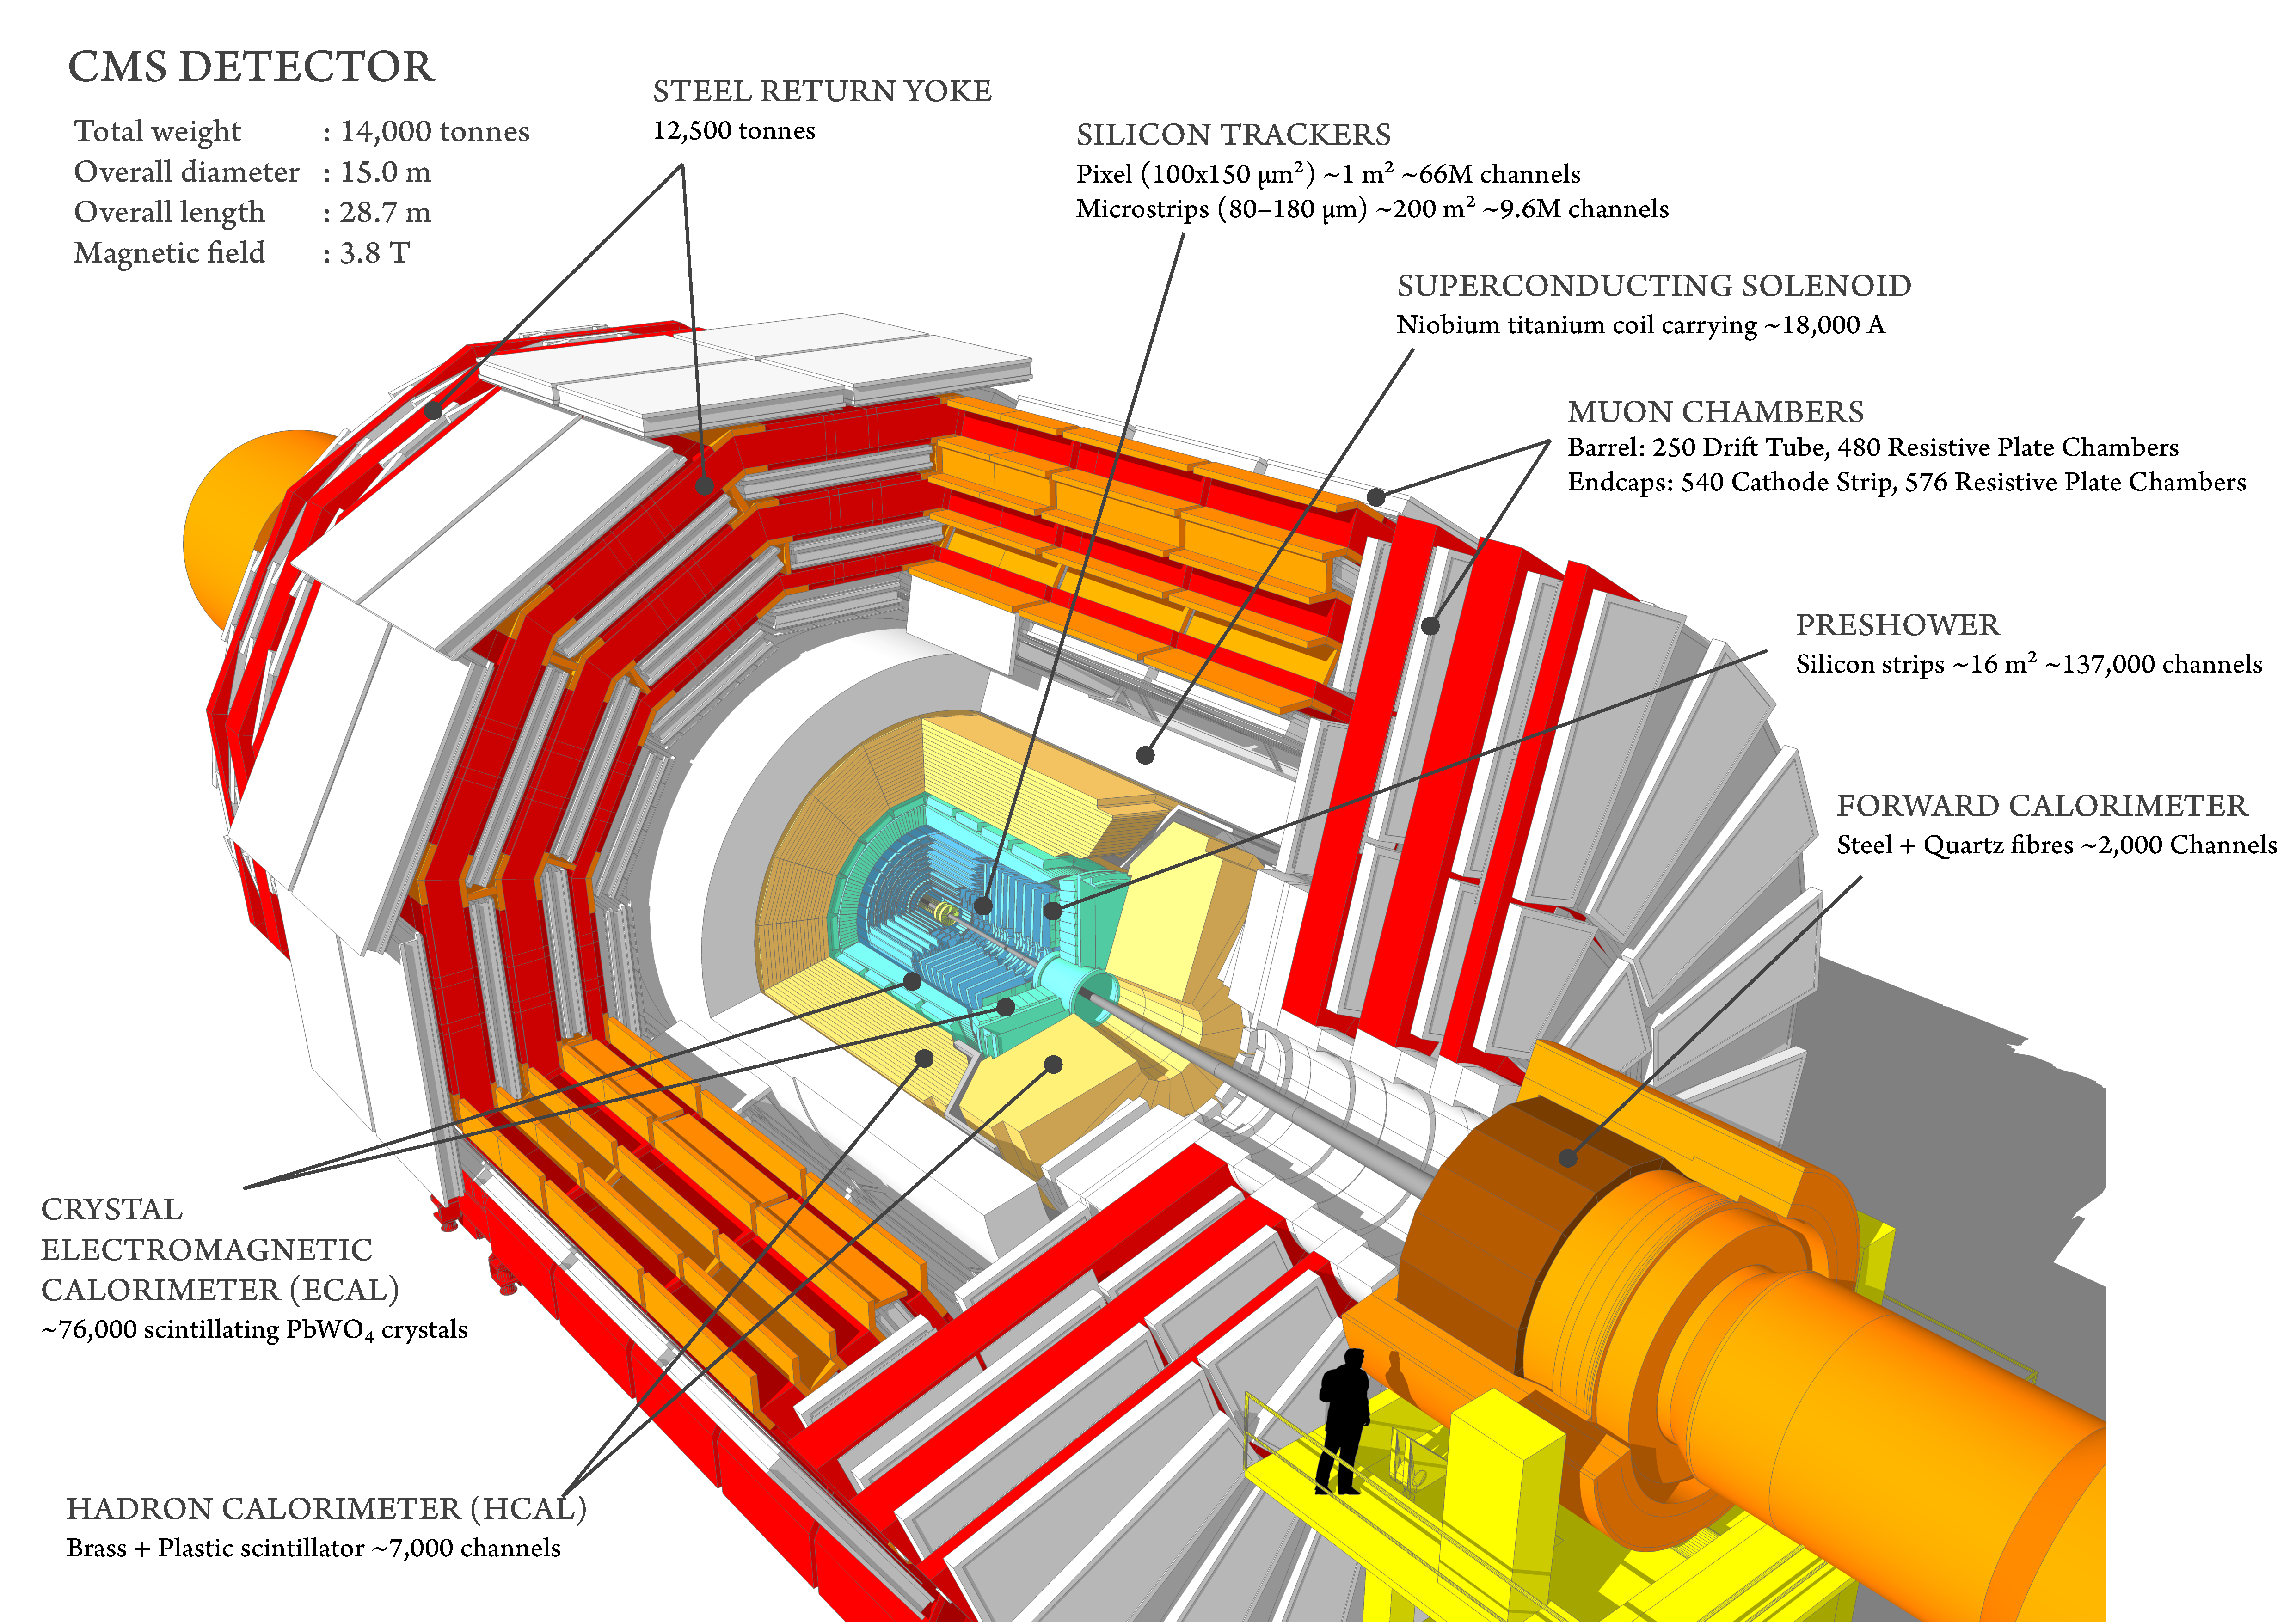
\includegraphics[width=0.9\textwidth]{figs/03_experiment/cms_160312_02.pdf}
	\caption[Cutaway diagram of CMS showcasing major detector components~\cite{Sakuma:2665537}.]
			{Cutaway diagram of CMS showcasing major detector components~\cite{Sakuma:2665537}.}
	\label{fig:CMS}
\end{figure}

\subsection{CMS Coordinate System} \label{sec:CMS_coord}
The origin of the CMS coordinate system is located at the center of the detector, at the nominal collision point of the proton beams. The $+\hat{x}$ axis points radially towards the center of the LHC, while the $+\hat{y}$ axis points vertically upward. This sets the $+\hat{z}$ direction along the beamline, counterclockwise along the LHC. Due to the cylindrical symmetry of CMS, coordinates in the $\hat{x}$-$\hat{y}$ plane are commonly replaced with the radius $r$ and the azimuthal angle $\phi$, which is measured from the positive $\hat{x}$-axis. The polar angle $\theta$ is measured from the $+\hat{z}$-axis, though in practice this variable is rarely used. It is more common to define the polar angle in terms of the pseudorapidity $\eta$, which is defined as
\begin{equation}
	\eta=\frac{1}{2}\ln\left(\frac{|\mathbf{p}|+p_{z}}{|\mathbf{p}|-p_{z}}\right)=-\ln{\tan\left(\frac{\theta}{2}\right)}
\end{equation}

The motivation for using $\eta$ instead of $\theta$ stems from a fundamental property of hadron colliders: the center of mass frame for particle production rarely coincides with the lab frame. Thus, when measuring the separation between particles, it is useful to define quantities that remain invariant under Lorentz transformations in the $\hat{z}$ direction. The rapidity $y$ (not to be confused with the Cartesian coordinate $\hat{y}$) is defined as
\begin{equation}
	y=\frac{1}{2}\ln\left(\frac{E+p_{z}}{E-p_{z}}\right)
\end{equation}
It is trivial to show that differences in $y$ remain invariant under Lorentz transformations. In the highly relativistic limit, which is valid for most particles produced at the LHC, rapidity approaches pseudorapidity as $E\approx|\mathbf{p}|$. One advantage of pseudorapidity is that $\eta$ can be calculated using only geometric quantities of the detector, whereas $y$ requires calculating both the energy and momenta of a particle, making pseudorapidity the natural choice for defining the polar angle. $\eta$ can range from $\left(-\infty, \infty\right)$, where $\eta=\pm\infty$ points directly along the $\pm\hat{z}$ axis. Higher values of $\left|\eta\right|$ are commonly referred to as "forward".

\subsection{Inner Tracker} \label{sec:CMS_tracker}
The CMS inner tracker is the first detector surrounding the primary interaction point (IP). Its purpose is to measure the tracks from charged particles as they curve in the strong magnetic field within CMS in order to calculate their momentum and reconstruct secondary vertices. As the closest detector to the primary IP, the tracker experiences the highest particle flux within CMS, and must have high enough granularity to distinguish the multitude of tracks. Additionally, particles passing through must lose minimal energy in order to maintain their trajectories into the outer detectors. The high flux also makes the detector susceptible to radiation damage, so the tracker must be robust in order to maintain efficiency over the long operational period of the LHC.

The inner tracker utilizes silicon tracking modules to detect the location of charged particles. When an external voltage is applied to a module, particles passing through will deposit energy and create electron-hole pairs, which drift to their respective electrodes and generate an electrical signal. The applied voltage is tuned such that only a small amount of energy is required to produce electron-hole pairs, which reduces the total amount of material required in order to minimize the energy loss of the charged particles. The inner layer of the tracker is composed of higher granularity pixel detectors, while the outer layer is composed of coarser silicon strips.

\subsubsection{Silicon Pixel Detector} \label{sec:CMS_pixel}
The pixel detector is comprised of 124 million silicon pixel sensors, each with an area of $100\times150\unit{\mu m^2}$ and a thickness of $300\unit{\mu m}$. The barrel (BPIX) consists of four cylindrical layers of pixel sensors spanning from $z=-54\unit{cm}$ to $z=54\unit{cm}$ at radii of $r=2.9$, $6.8$, $10.9$, and $16\unit{cm}$. The endcap (FPIX) consists of three layers located at $z=\pm29.1$, $\pm39.6$, and $\pm51.6\unit{cm}$, which when combined with the barrel nets a total sensitive area of $1.85\unit{m^2}$ with coverage up to $\abs{\eta}<2.5$. With regards to detector performance, the pixel detector provides spatial resolution of $9.5 \unit{\mu m}$ in the $r$-$\phi$ direction and $22.2 \unit{\mu m}$ in the $z$ direction, as well as a hit efficiency of $>99\%$ in each layer at nominal LHC luminosity, with the innermost BPIX layer dropping to $97.5\%$ at peak run 2 efficiency~\cite{CMSPixelP1}.

\begin{figure}[htbp]
	\centering
	\includegraphics[width=0.85\textwidth]{figs/03_experiment/20120828_01_pixel_phase1_largesharp.png}
	\caption
	[$r$-$z$ slice of the CMS pixel detector~\cite{CMSPixelP1}]
	{$r$-$z$ slice of the CMS pixel detector comparing original design (bottom, teal) with the Phase-I upgrade implemented in 2016/17, which added one layer to both the FPIX and BPIX (top, blue)~\cite{CMSPixelP1}.}
	\label{fig:pixel}
\end{figure}

\subsubsection{Silicon Strip Detector} \label{sec:CMS_strip}
The silicon strip detector surrounds the pixel detector, and is segmented into a tracker inner barrel (TIB), tracker outer barrel (TOB), tracker inner disks (TID), and tracker endcap (TEC). The TIB consists of four layers covering $\left|z\right|<65\unit{cm}$ and radius $25.5\unit{cm}<r<49.8\unit{cm}$. The endcaps of the TIB are covered by the TID, consisting of three disks covering $90<\left|z\right|<90\unit{cm}$. Surrounding the TIB is the TOB, with six layers spanning $\left|z\right|<188\unit{cm}$ and $60.8<\left|r\right|<108\unit{cm}$. Lastly, both the TOB and TID are closed by the TEC, which covers radii ranging from $22<r<113.5\unit{cm}$ and stretches from $124<\left|z\right|<280\unit{cm}$.

The strip detector modules function similarly to the pixel modules, but utilize much larger silicon strips due to the reduced particle flux compared to the pixel detector. Each strip detector is composed of $300\unit{\mu m}$ thick micro-strip sensors with pitch varying from $80-205\unit{\mu m}$ to form $7-12.5\unit{cm}$ long strip modules. Overall, the strip detector uses 15,148 modules covering an area of $200\unit{m^2}$ up to $\left|\eta\right|<2.5$.

\begin{figure}[htbp]
	\centering
	\includegraphics[width=0.85\textwidth]{figs/03_experiment/las.png}
	\caption
	[$r$-$z$ slice of the CMS silicon detector, detailing the four main components of the strip detector~\cite{Chatrchyan:1211825}]
	{$r$-$z$ slice of the CMS silicon detector, detailing the four main components (TIB, TOB, TID, and TEC) of the strip detector. Pixel detector is shown in its Run-I configuration~\cite{Chatrchyan:1211825}}
	\label{fig:strip}
\end{figure}

\subsection{Electromagnetic Calorimeter} \label{sec:CMS_ECAL}
The CMS Electromagnetic Calorimeter (ECAL) is designed to stop and capture the energy of photons and electrons. When a photon or election enters the ECAL, it interacts with the material in the detector through bremsstrahlung, $e^+e^-$ pair production, Compton scattering, or ionization, which in turn produce more photons or electseparaterons that continue these processes in a cascade that is referred to as an electromagnetic shower. The light produced from a shower is measured using photodetectors to determine the initial energy of the incident photon or electron, as the amount of light produced is proportional to the initial energy.

The material used for an electromagnetic calorimeter can be characterized by the radiation length ($X_0$) and moli\`ere radius ($R_M$). The radiation length is the average distance an electron will travel before its energy is reduced by a factor of $1/e$, and is roughly proportional to $A/Z^2$, where A is the atomic mass and Z is the atomic number. The moli\`ere radius directly proportional to the radiation length and measures the spread of an electromagnetic shower in the transverse direction. A low radiation length and moli\`ere radius ensure all of the energy is captured in the detector and is contained to a small area to precisely determine the position of an incident particle. It is for this reason that the CMS ECAL is composed of lead-tungstate (PbWO$_4$): a dense, high Z scintillator crystal with $X_0=7.39\unit{g/cm^2}$ (or $0.89\unit{cm}$ after dividing by the density of PbWO$_4$) and $R_M=2.2\unit{cm}$~\cite{Workman:2022ynf}.

The ECAL is constructed from 61200 + 15000 lead-tungstate crystals in the barrel + endcap region. Barrel crystals have a cross sectional area of $2.2\times2.2\unit{cm^2}$ to match the moli\`ere radius and a depth of 23$\unit{cm}$ (or $25.8 X_0$), and are arranged in rings along the $\phi$ direction, tilted to align with lines of constant $\eta$. The barrel has an inner radius of $129\unit{cm}$ and covers an eta region up to $\left|\eta\right|<1.479$. Endcap crystals have a slightly higher cross sectional area of $2.6\times2.6\unit{cm^2}$ and a slightly lower depth of 22$\unit{cm}$, and are arranged in an $x$-$y$ grid. The endcap provides the remaining coverage from $1.479<\left|\eta\right|<3.0$. Size and alignment of the crystals is designed to contain showers from incident photons/electrons within a $2\times2$ grid.

One common process in CMS is the production of $\pi^0$s, which decay to two photons. When the two photons deposit their energy into the ECAL, they can fake a signal from a single high energy photon. In the barrel, the two photons are generally separated by $\sim1\unit{cm}$, so the crystal granularity can be used to distinguish this background from real, high energy photons. However, $\pi^0$s in the forward region tend to be higher energy (commonly referred to as "more boosted"), resulting in separations on the order of millimeters. In order to identify these background events, a higher granularity detector known as a preshower is placed before the ECAL endcap. It consists of a layer of lead absorber to initiate the shower, followed by silicon strip sensors to measure the tracks within the shower. The lead has a thickness of $1.57\unit{cm}$ (or $2.8X_0$), thick enough to cause a shower while only causing energy loss of a few percent before the shower can reach the ECAL. The silicon strips are similar to those in the inner tracker, with a pitch of $1.9\unit{mm}$~\cite{TOURNEFIER2001355}.

\begin{figure}[htpb]
	\centering
	\includegraphics[width=0.85\textwidth]{figs/03_experiment/cms_ecal.pdf}
	\caption
	[Geometry of the CMS ECAL showing the barrel, endcap, and preshower, adapted from~\cite{Marzocchi2019}]
	{Geometry of the CMS ECAL showing the barrel, endcap, and preshower, adapted from~\cite{Marzocchi2019}}
	\label{fig:ecal}
\end{figure}


\subsection{Hadronic Calorimeter} \label{sec:CMS_HCAL}

\subsection{Muon Detectors} \label{sec:CMS_Muons}

\subsection{Trigger System} \label{sec:CMS_trig}

\subsubsection{Level-1 Trigger} \label{sec:CMS_L1T}

\subsubsection{High Level Trigger} \label{sec:CMS_HLT}

\subsection{Particle Flow} \label{sec:CMS_PF}